\section{Introduction}
\label{sec:introduction}
\begin{figure}[t]
    \centering
    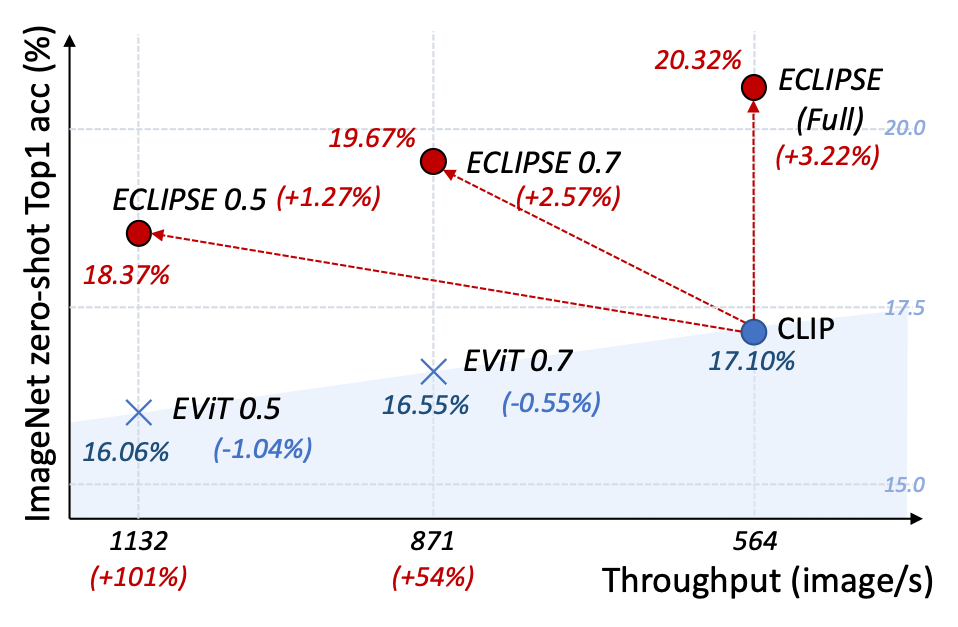
\includegraphics[width=0.9\columnwidth]{figures/imgs/figure_speed.png}
    \caption{Time vs. ImageNet zero-shot performance analysis for Contrastive Language-Image Pretraining with existing ViT accleration framework (EViT).
    We compare the results between EViT directly applied on CLIP and EViT trained with our proposed meta-architecture, ECLIPSE.
    Our proposed framework enables even streamlined ViTs with 101\% faster throughputs to outperform the full ViT of CLIP.
    Model performance and inference time are measured with ViT-B/16 backbone.
    }
    \label{fig:fig_speed}
\end{figure}
% Transformers in Computer vision
Transformers~\cite{vaswani2017attention} have achieved significant progress across various challenging vision tasks such as image classification~\cite{dosovitskiy2021an,touvron2021training,jiang2021all,graham2021levit}, object detection~\cite{carion2020end}, semantic segmentation~\cite{xie2021segformer,liu2021swin,wang2021pyramid} and visual relationship detection~\cite{kim2021hotr,kim2022mstr}.
% ViTs in Contrastive Language-Image Pretraining
Following this success in vision tasks, recent studies demonstrated that large-scale vision-language pretraining (VLP)~\cite{li2019visualbert,chen2019uniter,huang2019unicoder,li2020oscar,li2020unimo,lu2019vilbert,tan2019lxmert,jia2021scaling,radford2021learning} with ViTs is scalable to large uncurated datasets and transferable to various downstream tasks.

% Computational overhead of distillation
However, the large scale image-text pairs for VLP are usually collected from the web; thus they are often noisy, i.e., having weak correlation between the image and its corresponding text description.
To alleviate the image-text misalignment problem, previous works~\cite{li2021align,Lu2022COTS} have proposed knowledge distillation framework~\cite{hinton2015distilling} with a momentum encoder for both image and text.
However, adopting two additional momentum encoders and calculating soft alignments for distillation loss inevitably increase the computational cost for training, which hinders training for large-scale VLP.

% Efficient Distillation
In this work, we propose a efficient formulation for distilling soft image-text alignment matrix without text momentum encoder for contrastive language-image pretraining~\cite{jia2021scaling,radford2021learning}.
Inspired from SimSiam~\cite{chen2021exploring}, we simply replace the text momentum encoder with stop-gradient operation.
This design not only eliminates the computational cost for an additional text momentum encoder, but also enables the distillation to operate within a unified projected space of text embedding, resulting in better performance.
Based on this shared projected space, we adopt token sparsification~\cite{liang2022evit} for the online image encoder to i) provide a partial view that complementarily interacts with the full-view of the momentum image encoder, ii) compensate for the computational overhead of training the momentum image encoder, and iii) accelerate inference speed.
% Moreover, we further mitigate the heavy computational overhead by adopting token sparsification frameworks~\cite{liang2022evit} to expedite vision transformers which was originally proposed for supervised learning.
% Model acceleration can also improve inference speed unlike training acceleration via random masking of input patches~\cite{li2022scaling}.
% This unique design not only effectively improves data efficiency by alleviating the natural misalignment between images and text, but it also enhances computational efficiency by expediting online network.
While our distillation architecture effectively improves data efficiency by alleviating the natural misalignment between images and text, the expedited online image encoder and the momentum teacher positively interacts with a sweet spot that achieves speed improvement without degrading performance.
We name this meta-architecture as ECLIPSE: \textbf{E}xpediting \textbf{C}ontrastive \textbf{L}anguage-\textbf{I}mage \textbf{P}retraining with \textbf{S}elf-distilled \textbf{E}ncoders.
ECLIPSE is trained with a loss jointly obtained from two image-text alignment matrices (i.e., $\bar{A}$ and $A$ in Fig.~\ref{fig:fig_overview}):
\begin{itemize}
    \item The batch-wise image-text alignment matrix $\bar{A}$ between the text encoder and the momentum teacher is trained with an InfoNCE loss~\cite{oord2018representation} with hard alignment labels for matching image-text pairs.
    
    \item Student-text alignment matrix $A$ is obtained likewise with the online network and the text encoder with stop gradient. We train the online network to match $A$ with the soft alignment matrix $\bar{A}$ obtained above.
\end{itemize}
The momentum parameters are updated with an exponential moving average (EMA) of the parameters of online encoder.

Extensive experiments demonstrate the effectiveness of ECLIPSE, showing that our distillation architecture significantly improves data efficiency while achieving substantial model acceleration.
For example, when applied to CLIP~\cite{radford2021learning}, our proposed architecture improves 1.27\% zero-shot accuracy in ImageNet classification while achieving 101\% acceleration in inference speed.
Moreover, ECLIPSE can be also trained without expedition, which then shows a large 3.22\% gain compared to ViT, thus offers a model choice between an accelerated model with competitive performance and a full-capacity model with enhanced performance (see Fig.~\ref{fig:fig_speed} and Tab.~\ref{tab:keep}).
Furthermore, scaling to large-scale datasets, ECLIPSE achieves state-of-the-art on several downstream tasks, outperforming CLIP variants with a model accelerated by more than 54\%.

\begin{figure}
    \centering
    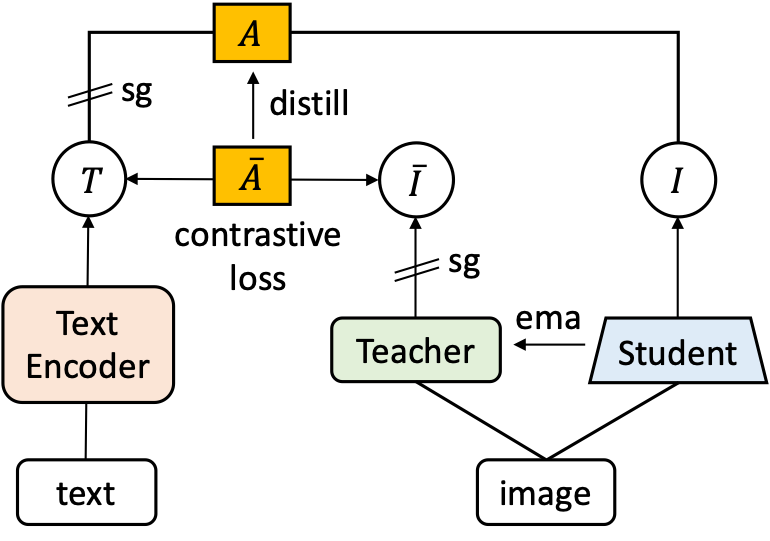
\includegraphics[width=0.8\columnwidth]{figures/imgs/figure_overview.png}
    \vspace{0.7em}
    \caption{Overview of ECLIPSE. Student encoder is trained to estimate the soft alignment matrix $\bar{A}$ predicted by Text Encoder and the Teacher network.
    sg stands for stop-gradient, $I$ and $\bar{I}$ are encoded image with student and teacher network, respectively.
    }
    \label{fig:fig_overview}
\end{figure}